\documentclass[17pt,a4paper,landscape]{extarticle}
\usepackage[margin=2.35cm,top=0.12cm,left=1.05cm]{geometry}
\usepackage{amsmath}
\usepackage{amssymb}
\usepackage{tasks}
\usepackage{tikz}
\usepackage{xcolor}
\usepackage[sfdefault,lf]{FiraSans}
\renewcommand{\familydefault}{\sfdefault}
\setlength{\parindent}{0pt}
\pagestyle{empty}
\settasks{label=\textbf{\arabic*.}, label-width=2.2em, item-indent=2.95em, column-sep=2.1cm, after-item-skip=4.7em}
\renewcommand{\arraystretch}{1.15}
\everymath{\displaystyle}

\begin{document}
\sffamily
\boldmath

\boldmath

\boldmath

\boldmath

\boldmath

{\Large \textbf{Perimeter (shapes with straight edges only) --- Excellence}}
\begin{tasks}(3)
\task Find the perimeter.\\[0.4em]
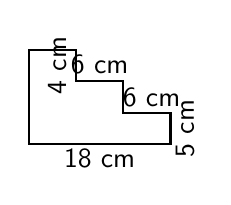
\begin{tikzpicture}[x=0.20cm,y=0.20cm,baseline=(current bounding box.center)]
  \draw[thick] (0,0)--(9,0)--(9,2)--(6,2)--(6,4)--(3,4)--(3,6)--(0,6)--cycle;
  \node at (4.5,-0.9) {18 cm};
  \node[rotate=90] at (9.9,1) {5 cm};
  \node at (7.8,3.0) {6 cm};
  \node at (4.5,5.1) {6 cm};
  \node[rotate=90] at (1.8,5) {4 cm};
\end{tikzpicture}
\task Find the perimeter.\\[0.4em]
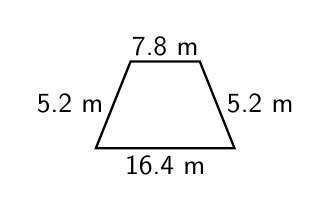
\begin{tikzpicture}[x=0.22cm,y=0.22cm,baseline=(current bounding box.center)]
  \draw[thick] (0,0)--(8,0)--(6,5)--(2,5)--cycle;
  \node at (4,-1.0) {16.4 m};
  \node at (4,5.9) {7.8 m};
  \node at (1.0,2.6) [left] {5.2 m};
  \node at (7.0,2.6) [right] {5.2 m};
\end{tikzpicture}
\task Find the perimeter.\\[0.4em]
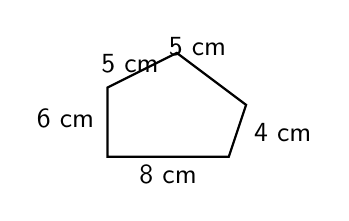
\begin{tikzpicture}[x=0.22cm,y=0.22cm,baseline=(current bounding box.center)]
  \draw[thick] (0,0)--(7,0)--(8,3)--(4,6)--(0,4)--cycle;
  \node at (3.5,-1.0) {8 cm};
  \node at (7.9,1.4) [right] {4 cm};
  \node at (5.2,6.4) {5 cm};
  \node at (-0.2,2.2) [left] {6 cm};
  \node at (1.3,5.4) {5 cm};
\end{tikzpicture}
\task Find the perimeter.\\[0.4em]
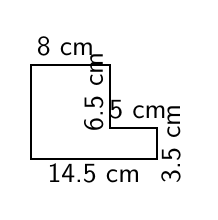
\begin{tikzpicture}[x=0.20cm,y=0.20cm,baseline=(current bounding box.center)]
  \draw[thick] (0,0)--(8,0)--(8,2)--(5,2)--(5,6)--(0,6)--cycle;
  \node at (4,-0.9) {14.5 cm};
  \node[rotate=90] at (8.9,1) {3.5 cm};
  \node at (6.8,3.2) {5 cm};
  \node[rotate=90] at (4.0,4.3) {6.5 cm};
  \node at (2.2,7.2) {8 cm};
\end{tikzpicture}
\task The perimeter of a rectangle is 52 cm. Its length is 4 cm more than its width. Find both dimensions.
\task An isosceles triangle has perimeter 31 cm. The equal sides are 9 cm each. Find the third side.
\task A square and a rectangle both have perimeter 24 cm. The square has side 6 cm. Give one possible pair of whole-number dimensions for the rectangle that is not a square.
\task Maia walks once around a field shaped like a trapezium with sides 42 m, 35 m, 28 m and 35 m. How far does she walk in 3 laps?
\task A rectangle is widened by 3 cm and its perimeter increases by 6 cm. Explain why this always happens.
\task Which has the greater perimeter: a \mbox{$7$} cm by \mbox{$11$} cm rectangle or a triangle with sides \mbox{$8$} cm, \mbox{$9$} cm and \mbox{$12$} cm? How much greater?
\task A regular pentagon has perimeter 47.5 cm. Find one side length.
\task A builder used \mbox{$36$} m of timber around the edge of a rectangular deck. If the width is \mbox{$7$} m, find the length.
\end{tasks}

\end{document}
